\documentclass[a4paper,12pt]{article}
\pagestyle{empty}
\usepackage[left=2cm,right=2cm,
    top=2cm,bottom=2cm,bindingoffset=0cm]{geometry}
%%% Работа с русским языком
\usepackage{cmap}					% поиск в PDF
\usepackage{mathtext} 				% русские буквы в формулах
\usepackage[T2A]{fontenc}			% кодировка
\usepackage[utf8]{inputenc}			% кодировка исходного текста
\usepackage[english,russian]{babel}	% локализация и переносы
\usepackage{xcolor}
\usepackage{hyperref}
 % Цвета для гиперссылок
\definecolor{linkcolor}{HTML}{799B03} % цвет ссылок
\definecolor{urlcolor}{HTML}{799B03} % цвет гиперссылок

\hypersetup{pdfstartview=FitH,  linkcolor=linkcolor,urlcolor=urlcolor, colorlinks=true}

%%% Дополнительная работа с математикой
\usepackage{amsfonts,amssymb,amsthm,mathtools} % AMS
\usepackage{amsmath}
\usepackage{icomma} % "Умная" запятая: $0,2$ --- число, $0, 2$ --- перечисление

%% Номера формул
%\mathtoolsset{showonlyrefs=true} % Показывать номера только у тех формул, на которые есть \eqref{} в тексте.

%% Шрифты
\usepackage{euscript}	 % Шрифт Евклид
\usepackage{mathrsfs} % Красивый матшрифт

%% Свои команды
\DeclareMathOperator{\sgn}{\mathop{sgn}}

%% Перенос знаков в формулах (по Львовскому)
\newcommand*{\hm}[1]{#1\nobreak\discretionary{}
{\hbox{$\mathsurround=0pt #1$}}{}}
% графика
\usepackage{graphicx}
\graphicspath{{pictures/}}
\DeclareGraphicsExtensions{.pdf,.png,.jpg}
\author{Бурмашев Григорий, БПМИ-208}
\title{Матан, дз -- 11 }
\date{\today}
\begin{document}
\maketitle
\begin{center}
\textbf{С НОВЫМ ГОДОМ!!!!!!!!!!!!!}
\end{center}
\begin{center}

\includegraphics[scale=0.3]{5.jpg}
\end{center}
\clearpage
{\Large \begin{center}
\textbf{А это мой кот, пусть будет тут }
\end{center}}
\begin{center}

\includegraphics[scale=0.4]{6.jpg}
\end{center}
\clearpage
\section*{Номер 1}
\[
\iint\limits_D \frac{(x+y)^2}{x}dxdy, \; \; D = \left\{(x, y) \Big| 1 -x \leq y \leq 3 - x , \frac{x}{2} \leq y \leq 2x \right\}
\]
Рисуем графичек по неравенствам:
\begin{center}
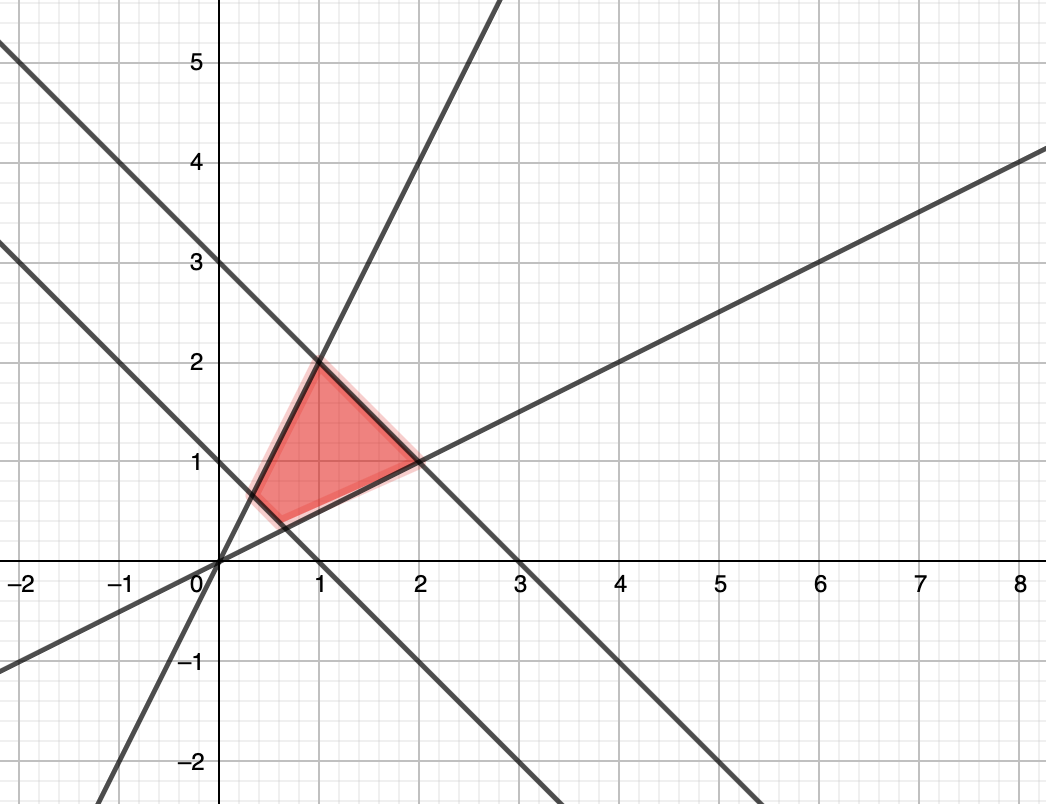
\includegraphics[scale=0.7]{1.png}
\end{center}
\begin{center}
Посмотрим на множество $D$:
\end{center}
Смотрим на первое неравенство:
\[
1 - x \leq y \leq 3 -x
\]
\[
 1 \leq x + y \leq 3
\]
Пусть $u = x + y$, тогда:
\[
1 \leq u \leq 3
\]
Смотрим на второе неравенство:
\[
\frac{x}{2} \leq y \leq 2x
\]
\[
\frac12 \leq \frac{y}{x} \leq 2
\]
Пусть $v = \frac{y}{x}$, тогда:
\[
\frac12 \leq v \leq 2
\]
Итого:
\[
\begin{cases}
u = x + y, u \in [1, 3]
\\
v = \frac{y}{x}, v \in \left[\frac{1}{2}, 2\right] 
\end{cases}
\]
\clearpage
А на графике в новых координатах получаем прямоугольник:
\begin{center}

\includegraphics[scale=0.4]{2.png}
\end{center}
Теперь считаем интеграл:

В числителе просто $u^2$, а вот в знаменателе у нас $x$, нужно его как-то выразить через новые координаты:
\[
y = vx
\]
\[
u = x + vx
\]
\[
\begin{cases}
x = \frac{u}{1 + v}
\\
y = \frac{uv}{1 + v}
\end{cases}
\]
Тогда определитель матрицы Якоби:
\[
\det \mathbb{J} = \begin{vmatrix}
\frac{1}{1 + v} & \frac{-u}{(1+v)^2} \\ \frac{v}{1+v} & \frac{u}{(1+v)^2}
\end{vmatrix} =
\frac{u}{(1+v)^3} + \frac{uv}{(1+v)^3} = \frac{u(1 + v)}{(1+v)^3} = \frac{u}{(1+v)^2}
\]
Теперь наконец считаем исходный интеграл в новых координатах:
\[
\iint\limits_{\begin{matrix} u \in [1, 3]\\ v \in \left[\frac12, 2\right]\end{matrix}} \left( \frac{u^2}{\frac{u}{1+v}} \cdot \frac{u}{(1+v)^2} \right)du dv =
\]
\[
=
\int_1^3 du \int_{\frac12}^2 \frac{u^2(1+v)}{u} \cdot \frac{u}{(1+v)^2} dv = \int_1^3 du \int_{\frac12}^2 \frac{u^2}{1} \cdot \frac{1}{(1+v)} dv  =\int_1^3 u^2 du \int_{\frac12}^2 \frac{1}{(1+v)} dv  = 
\]
\[
= \frac{26}{3}\int_{\frac12}^2 \frac{1}{(1+v)} dv  = \frac{26}{3} \ln |1 + v| \Bigg|_{\frac{1}{2}}^2 = \frac{26}{3} \left( \ln(3) - \ln\left(\frac{3}{2}\right)\right) = 
\]
\[
=
\frac{26}{3} \ln 2
\]
\begin{center}
\textbf{Ответ: } 
\[
\iint\limits_D \frac{(x+y)^2}{x}dxdy = \frac{26}{3} \ln 2
\]
\end{center}
\clearpage
\section*{Номер 2}
\[
\iiint\limits_D  z^2 dxdydz, \; D = \left\{ (x, y, z) \big| x^2 + y^2 + z^2 \geq 1, x^2 + y^2 + z^2 \leq 2z \right\}
\]
Теория с семинара:
\begin{center}
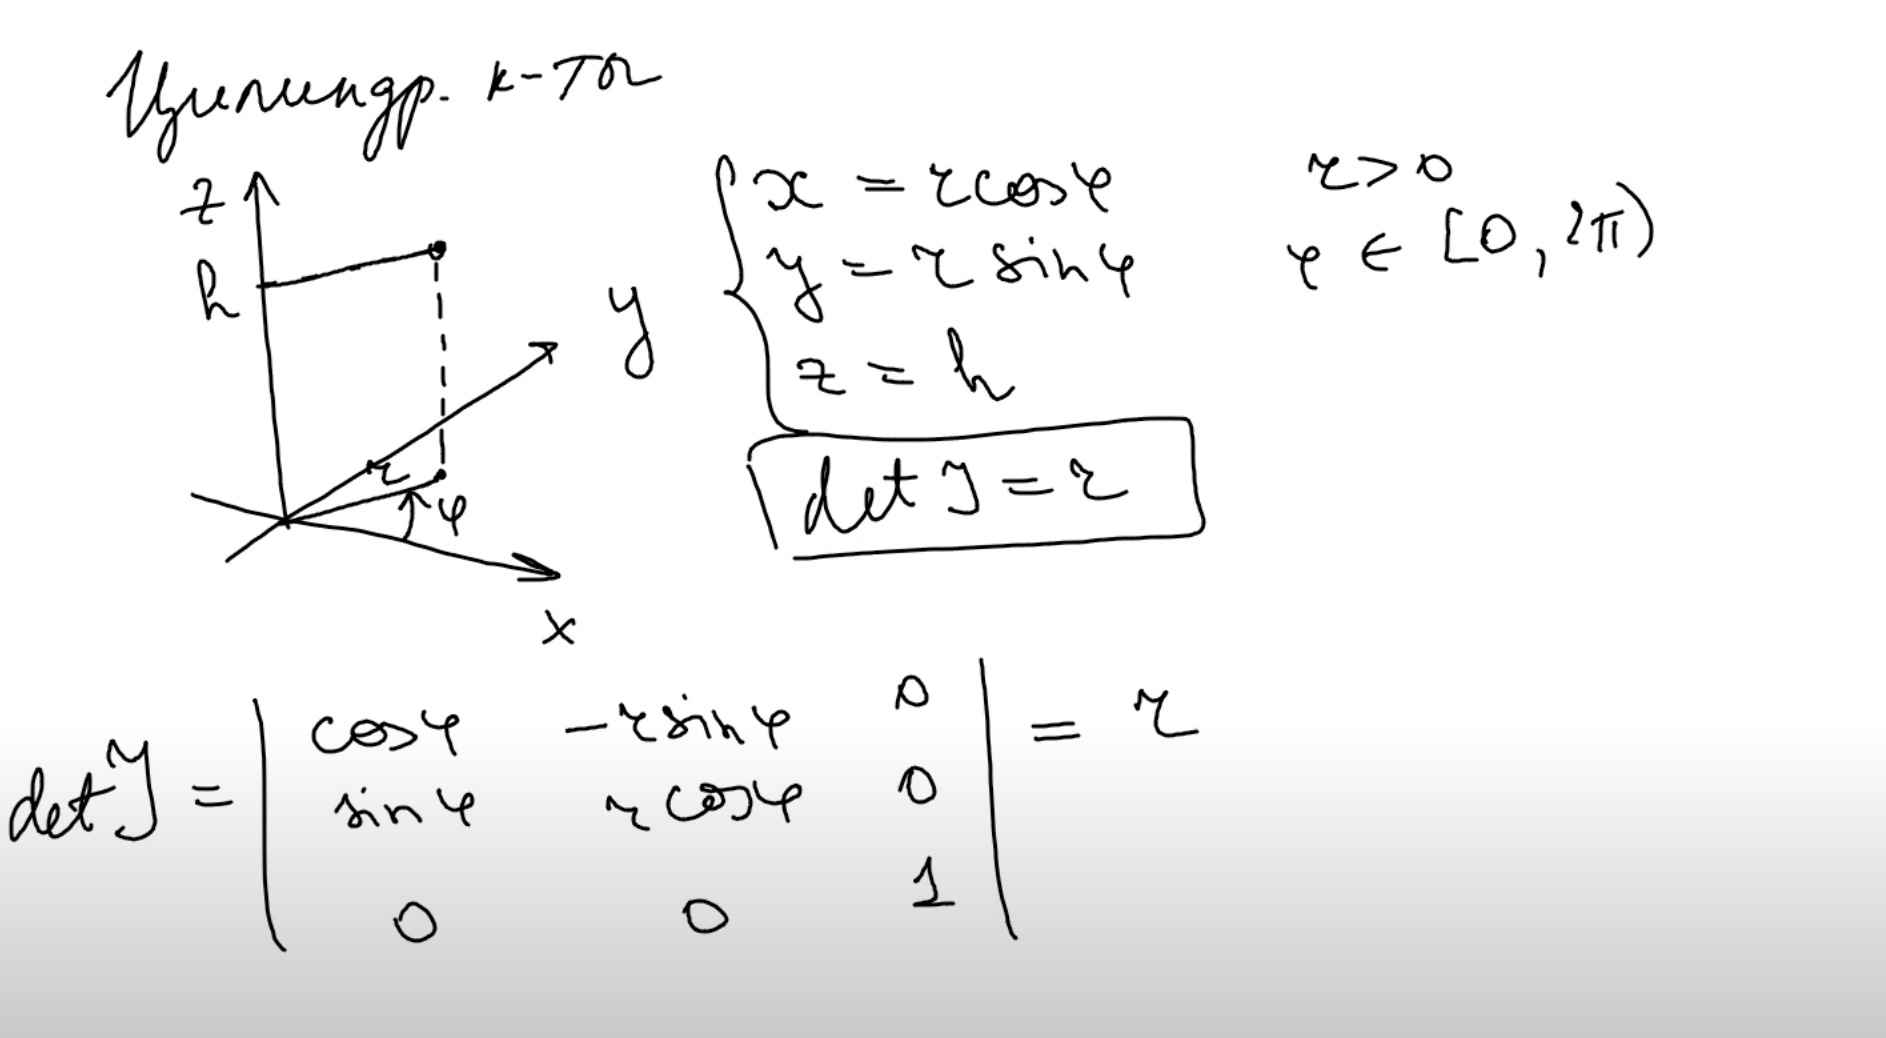
\includegraphics[scale=0.4]{3.png}
\end{center}
Тогда вводим цилиндрические координаты:
\[
\begin{cases}
r^2 + h^2 \geq 1 \\
r^2 + h^2 \leq 2h \\
r > 0, \varphi \in [0, 2\pi)
\end{cases}
\]
Для удобства рисования графика преобразуем второе неравенство:
\[
r^2 + h^2 \leq 2h \equiv r^2 + (h - 1)^2 \leq 1
\]
На графике имеем:
\begin{center}
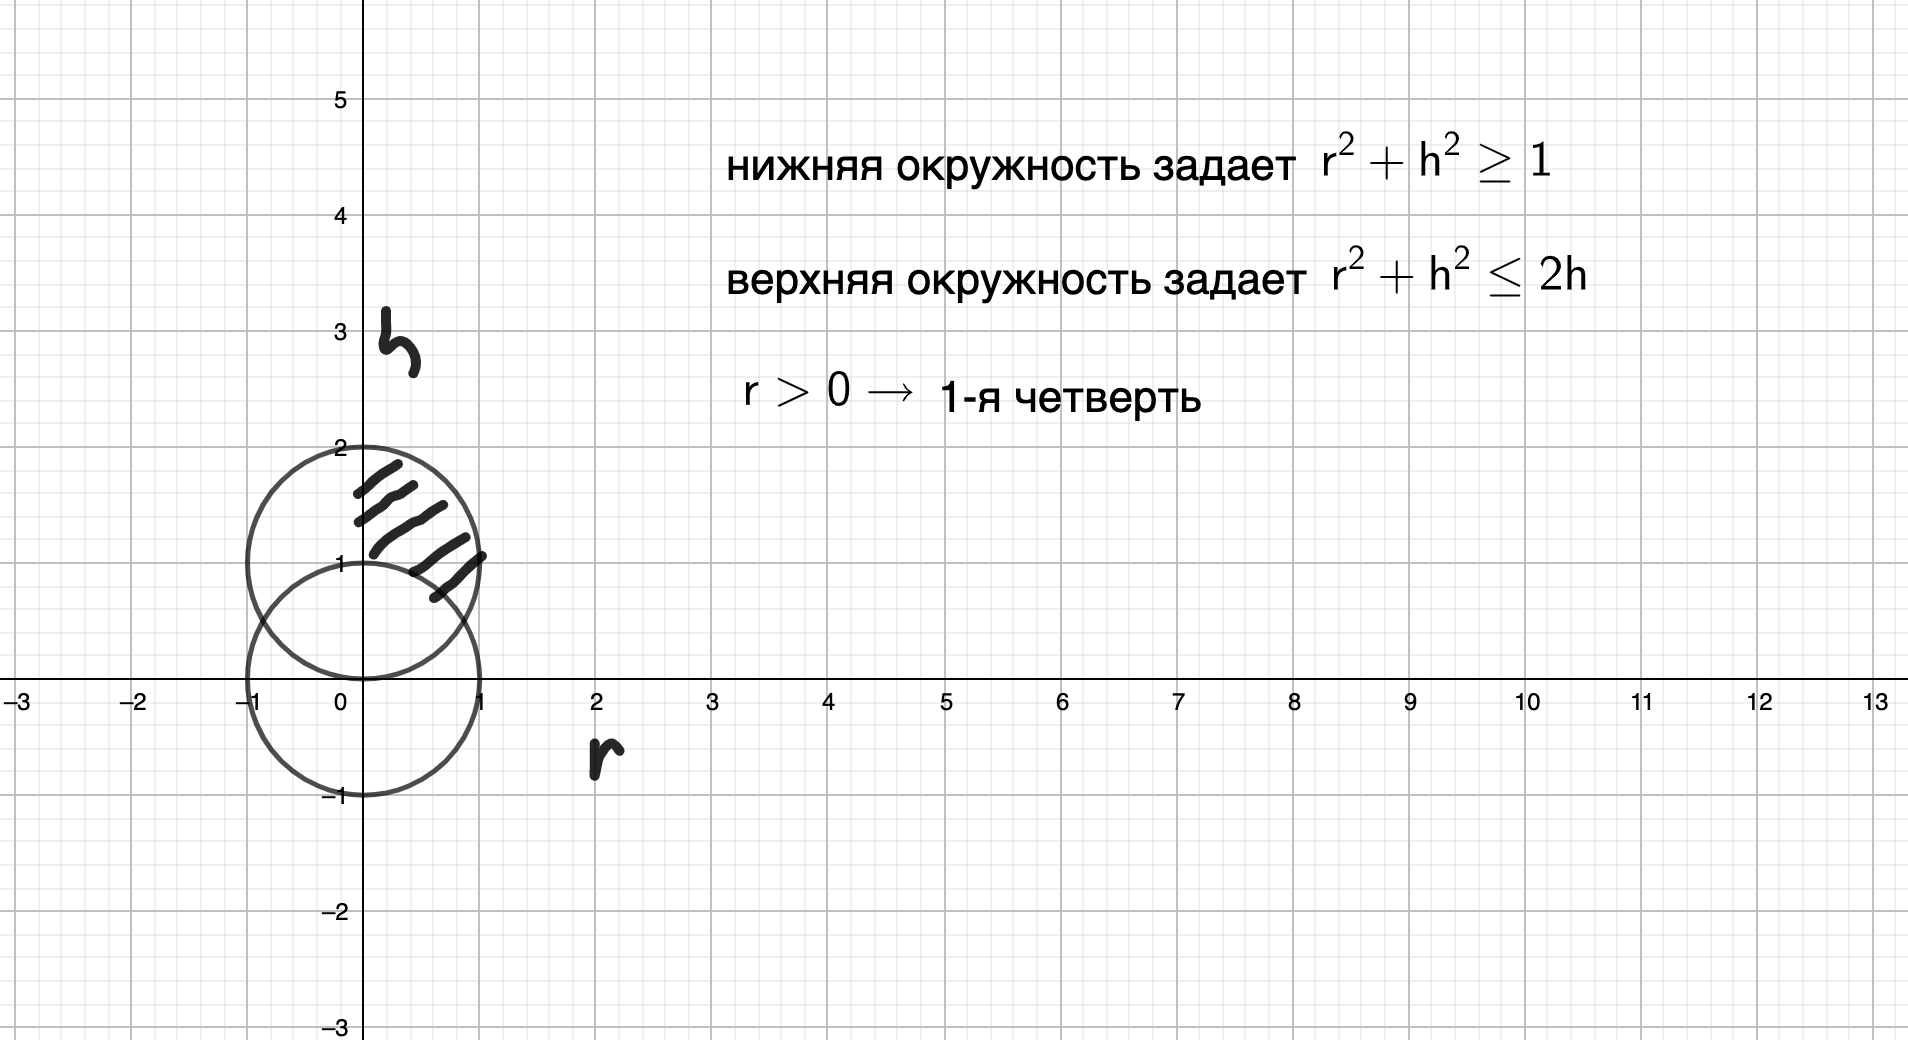
\includegraphics[scale=0.3]{4.png}
\end{center}
Из $r^2 + h^2 = 1$ получаем $h = \sqrt{1 - r^2}$, для верхней окружности соответственно $h = \sqrt{1 -r^2} + 1$
\\
Теперь считаем интеграл в новых координатах:
\[
 \int_0^{2\pi} d \varphi \int_0^1 r dr \int_{\sqrt{1-r^2}}^{\sqrt{1-r^2}+1}h^2 dh  = \int_0^{2\pi} d \varphi \int_0^1 r dr  \cdot \frac{h^3}{3} \Bigg|_{\sqrt{1-r^2}}^{\sqrt{1-r^2}+1} = 
\]
\[
=
\int_0^{2\pi} d \varphi \int_0^1 r dr  \cdot \frac{1}{3} \left( \left( \sqrt{1-r^2} + 1\right)^3 - \left(\sqrt{1-r^2}\right)^3 \right) =
\]
\[
=
\frac13 \int_0^{2\pi} d \varphi \int_0^1 r \left( \left( \sqrt{1-r^2} + 1\right)^3 - \left(\sqrt{1-r^2}\right)^3 \right)  dr = 
\]
\[
=
\frac13 \int_0^{2\pi} d \varphi \int_0^1 \left( 4r - 3 r^3 + 3r \sqrt{1 - r^2}\right)  dr = A
\]
Посчитаем внутренний интеграл отдельно:
\[
\int_0^1 4r dr =  4 \int_0^1 r dr  = 4 \cdot \frac{1}{2} = 2
\]
\[
\int_0^1 -3r^3dr = -3 \int_0^1 r^3 dr = -3 \cdot \frac14 = -\frac34
\]
\[
\int_0^1 3r \cdot  \sqrt{1-r^2} dr =  3 \int_0^1 r \cdot  \sqrt{1-r^2} dr  = \begin{bmatrix} t = 1 - r^2 \\ dt = -2rdr \end{bmatrix} = \frac32 \int_0^1 \sqrt{t}dt =\frac32 \cdot \frac23 = 1
\]
\[
2 - \frac34 + 1 = \frac94
\]
\[
A = 
 \frac13 \int_0^{2\pi} d \varphi \frac{9}{4} = \frac{3}{4}\int_0^{2\pi} d \varphi = \frac{3}{4} \cdot 2\pi  = \frac{3\pi}{2}
\]
В этот момент я решил, что это конечный ответ и пошел сверяться с вольфрамом и geogebra. Но при рисовании графиков в новых координатах я понял, что из-за наглого взятия  $r$ от 0 до 1 я зацепил лишний кусок справа под верхней окружностью :(. Хорошим вариантом было бы заново посчитать интеграл, разбив его на 2 части, но я не хочу переделывать все с нуля, поэтому просто вычту из интеграла $A$ схожий интеграл, который и отвечает за маленький кусочек площади. По $h$ он пройдет от $\sqrt{1-r^2}$ до $1 - \sqrt{1-r^2}$
 По $r$ он будет пробегать от точки пересечения окружностей при $r > 0$ и до 1, а точка пересечения:
\[
1 - \sqrt{1-r^2} = \sqrt{1-r^2} \;  (r > 0)
\]
\[
\frac{1}{2} = \sqrt{1-r^2}
\]
\[
r = \frac{\sqrt{3}}{2}  
\]
Теперь собственно считаем второй интеграл, пусть он будет B:
\[
B = \int_0^{2\pi} d \varphi \int_{\frac{\sqrt{3}}{2}}^1 rdr \int_{\sqrt{1-r^2}}^{1 - \sqrt{1-r^2}} h^2 dh =\int_0^{2\pi} d \varphi \int_{\frac{\sqrt{3}}{2}}^1 rdr \frac{h^3}{3} \Bigg|_{\sqrt{1-r^2}}^{1 - \sqrt{1-r^2}} =
\]
\[
= \frac{1}{3}\int_0^{2\pi} d \varphi \int_{\frac{\sqrt{3}}{2}}^1 rdr \left(  
\left(
1 - \sqrt{1-r^2}
\right)^3
-
\left(
\sqrt{1-r^2}
\right)^3
\right) =
\]
\[
\frac{1}{3}\int_0^{2\pi} d \varphi \int_{\frac{\sqrt{3}}{2}}^1 \left(
4 r - 3 r^3 - 5 r \sqrt{1 - r^2} + 2 r^3 \sqrt{1 - r^2} \right)dr = 
\]
Интегралы получились схожими со случаем для интеграла A, просто немного меняются коэффы и интервал интегрирования, лень техать это, оставлю на бумаге (надеюсь это не считается как необходимая подробность):
\[
=
 \frac{1}{3}\int_0^{2\pi}  \left(\frac{1}{2} - \frac{21}{64} - \frac{5}{24} + \frac{17}{240}
\right) d \varphi = \frac{1}{3}\int_0^{2\pi}   \frac{11}{320}d \varphi = \frac{1}{3} \cdot \frac{11}{320} \cdot 2\pi =  \frac{11\pi}{480}
\]
Теперь (\textbf{наконец-то, я умер техать это}) cчитаем финальный интеграл как разность интегралов A и B:
\[
\iiint\limits_D  z^2 dxdydz = A - B = \frac{3\pi}{2} -\frac{11\pi}{480} = \frac{709\pi}{480}
\]
\begin{center}
\textbf{Ответ: } 
\[
\iiint\limits_D  z^2 dxdydz =  \frac{709\pi}{480}
\]
\end{center}
\clearpage
{\Large \begin{center}
\textbf{И еще немного кота!}
\end{center}}
\begin{center}

\includegraphics[scale=0.5]{9.jpg}
\end{center}
\begin{center}

\includegraphics[scale=0.5]{8.jpg}
\end{center}
\begin{center}

\includegraphics[scale=0.6]{7.jpg}
\end{center}


\end{document}
